\clearpage



\begin{Indent}
  Fermi liquids are characterized by having $Z_{\bm k} > 0$ at the Fermi level!
\end{Indent}
It is a bit complicated to calculate~$\Sigma$ (see the integral expression in a previous chapter).
We will not perform the calculations here, but note that when the perturbation is the Coulomb potential, then the result is
\[
  \Sigma_I = -A_{\bm k}\, \mathrm{sgn}(\omega-\epsilon_F) (\omega-\epsilon_F)^2 = \Sigma_I(\bm k, \omega) \,,
\]
where $A_{\bm k} > 0$.
When $\omega \rightarrow \epsilon_F$, then $\Sigma_I \rightarrow 0$ as $(\omega-\epsilon_F)^2$:

\begin{figure}[H]
  \centering
  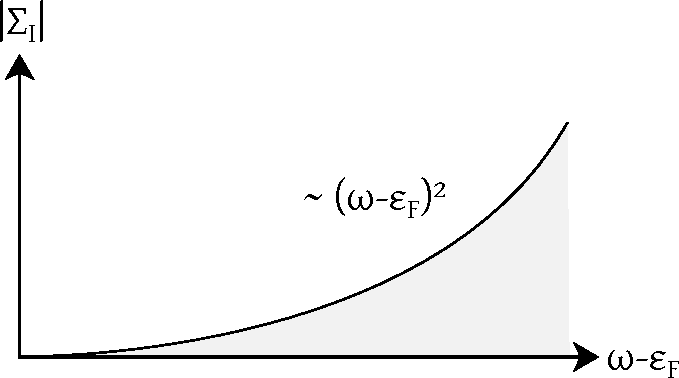
\includegraphics[width=0.5\textwidth]{img/pp181-200_selfenergy.pdf}
\end{figure}

The quasiparticles are well-defined close to the Fermi level because the damping is small.
If we get $\Sigma_I \sim (\omega-\epsilon_F)^2$, $\alpha < 1$, the damping disappears too slow, and $\alpha < 1$ is an indication that this is \emph{not} a Fermi liquid.
Finding a theoretical foundation for \emph{non}-Fermi liquid theory in $D>1$ dimensions is one of the big challenges in theoretical physics today (1995), since the normal ($T>T_c$) metallic state of high-$T_c$ superconductors exhibit transport properties that cannot be described as a Fermi liquid.
This may possibly be related to two-dimensional physics.

\emph{Heavy-fermion systems} (e.g. \ce{UPt3}): Correlation (Coulomb) effects are so large that the quasiparticles have masses $m^x/m \sim 1000$, and yet we have $Z_{k_F} > 0$!

3D: Fermi liquid theory is incredibly robust.

2D: ???

1D: Does not work, there is new physics here.



\clearpage
\section{Superconductivity}
The perturbation theory we have considered so far is well equipped to describe \emph{quantitative} changes in e.g. electron systems caused by many-particle effects.
Pure perturbation theory is not well suited to describe qualitative changes in a fermion or boson system caused by many-particle effects.
Examples of such qualitative changes may be:
\begin{enumerate}[(i)]
  \item Melting;
  \item Bose--Einstein condensation;
  \item Metal $\leftrightarrow$ insulator transitions;
  \item Metal/insulator  $\leftrightarrow$ superconductor transitions;
  \item Paramagnetic $\leftrightarrow$ ferromagnetic/antiferromagnetic transitions;
  \item Uniform electron gas $\leftrightarrow$ electron lattice (Wigner crystal) at low electron densities.
\end{enumerate}
Let $H$ be defined by:
\[
  H = H_0 + V
\]
$H_0$ can e.g. describe a simple metal in in case~(iv), or a paramagnet in case~(v).



\clearpage


\begin{figure}[H]
  \centering
  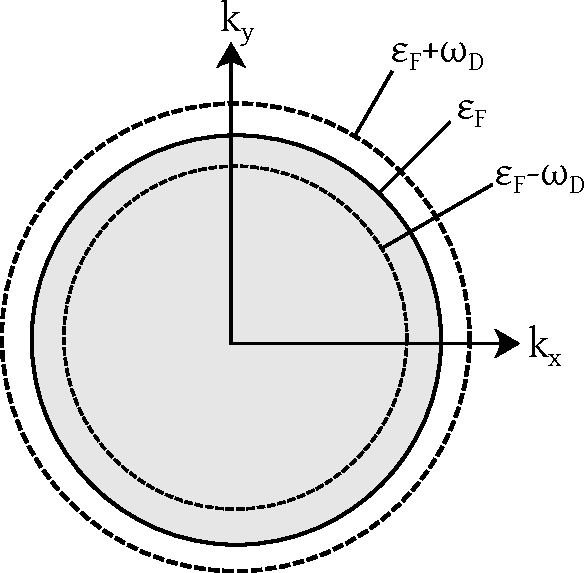
\includegraphics[width=0.5\textwidth]{img/pp181-200_fermisurface.pdf}
\end{figure}


\begin{figure}[H]
  \centering
  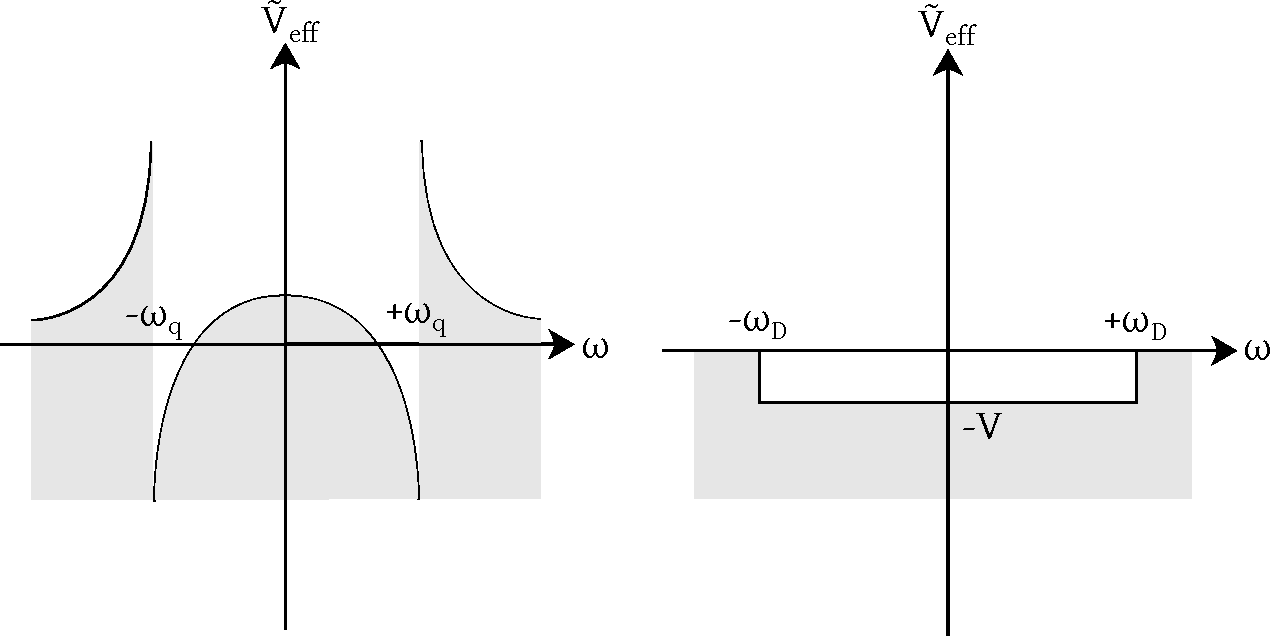
\includegraphics[width=\textwidth]{img/pp181-200_veffapprox.pdf}
\end{figure}



\begin{figure}[H]
  \centering
  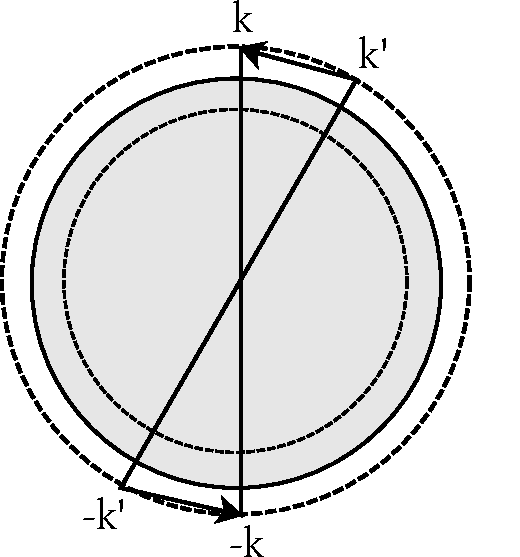
\includegraphics[width=0.45\textwidth]{img/pp181-200_coopermodel.pdf}
\end{figure}


\begin{figure}[H]
  \centering
  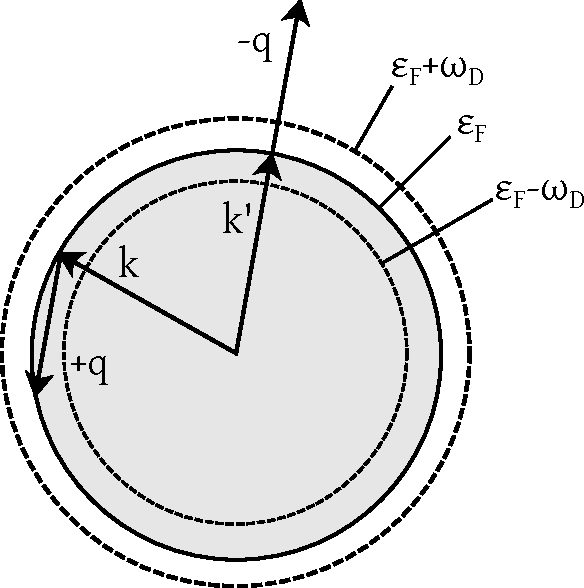
\includegraphics[width=0.5\textwidth]{img/pp181-200_cooperlimits.pdf}
\end{figure}
